\section{Non-equilibrium modeling}

\subsection{General Model}

In this section, we derive a general non-equilibrium kinetic model used for fitting the MWT data and viability modeling. We consider in the rate of change of the electron density \(n_{e}\) in time, given by

\begin{equation}
  \label{eq:start_deqn}
\frac{dn_{e}}{dt} = G - R,
\end{equation}
where \(G\) is the generation rate of electrons and \(R\) is the recombination rate. We consider the generation rate to be comprised of a thermal generation rate and a non-equilibrium generation rate, given by

\begin{equation}
  G = G_{th} + G_{NE},
\end{equation}
where \(G_{th}\) is the thermal generation rate constant and \(G_{NE}\) is the non-equilibrium generation rate. 

The recombination rate can be written

\begin{equation}
  R = - \sum_{i}^{}k_{r, b, i}n_{e}n_{i},
\end{equation}

Where $k_{r, b, i}$ [\unit{\centi\meter^3/\second}] and $n_i$ [\unit{1/\centi/\meter^3}] are the bimolecular recombination rate constant and species density $[1/cm^3]$ for the \emph{i}\textsuperscript{th} species, respectively. 

We consider the system under a perturbation from equilibrium, and write $n_i$ as the equilibrium density plus a perturbation, given by

\begin{equation}
  n_{i} = n_{i,0} + \Delta n_{i},
\end{equation}
with an identical equation for the electron density. We can then write the recombination rate as

\begin{equation}
  R = - \sum_{i}^{}k_{r, b, i}(n_{e,0} + \Delta n_{e})(n_{i,0} + \Delta n_{i}),
\end{equation}
which becomes

\begin{equation}
  \label{eq:recomb_expand}
  R = - \sum_{i}^{}[k_{r, b, i}n_{e,0}n_{i,0}  + k_{r, b, i}n_{i,0}\Delta n_{e} + k_{r, b, i}n_{e,0}\Delta n_{i} + k_{r, b, i}\Delta n_{e}\Delta n_{i}]
\end{equation}
after expansion of the product.

If we consider Equation \ref{eq:start_deqn} in the equilibrium case where $\frac{dn_{e}}{dt} = 0$ and $G_{NE} = 0$, we can see that the first term in Eq.\ \ref{eq:recomb_expand} is equal to $G_{th}$. Therefore, this term will cancel out in Eq.\ \ref{eq:start_deqn}, and we can write the full differential equation as

\begin{equation}
  \label{eq:full_deqn}
\frac{d\Delta n_{e}}{dt} = G_{NE}  -  \sum_{i}^{}[k_{r, b, i}n_{i,0}\Delta n_{e} + k_{r, b, i}n_{e,0}\Delta n_{i} + k_{r, b, i}\Delta n_{e}\Delta n_{i}].
\end{equation}

We assume that $\Delta n_i$ is proportional to $\Delta n_e$ — $\Delta n_i = \phi_i \Delta n_{e}$ — where $\phi_i$ is a proportionality constant. This assumption is motivated by the fact that $\Delta n_i$ and $\Delta n_e$ are created from the same non-equilibrium process. The focus of our analysis is for small perturbations from equilibrium (discussed below), and we assume that the relationship between any created $\Delta n_i$ and $\Delta n_e$ can be linearized. We can then substitute this into Equation \ref{eq:full_deqn} to get

\begin{equation}
  \label{eq:full_deqn_phi}
\frac{d\Delta n_{e}}{dt} = G_{NE} - k_{r, m, eff}\Delta n_{e} - k_{r, b, eff} \Delta n_{e}^2,
\end{equation}
where we have defined the effective mono-molecular recombination rate constant, $k_{r, m, eff}$, and effective bimolecular recombination rate constant, $k_{r, b, eff}$, as


\begin{equation}
\label{eq:krm_eff_def}
k_{r, m, eff} = \sum_{i}^{}k_{r, b, i}[n_{i,0} + n_{e,0}\phi_i]
\end{equation}
and
\begin{equation}
\label{eq:krb_eff_def}
k_{r, b, eff} = \sum_{i}^{}k_{r, b, i}\phi_i.
\end{equation}
For small enough $\Delta n_e$, the second (bimolecular) term in Equation \ref{eq:full_deqn_phi} can be neglected, giving

\begin{equation}
  \label{eq:small_pert_diffeq}
\frac{d\Delta n_{e}}{dt} = G_{NE} - k_{r,m,eff} \Delta n_{e}
\end{equation}
for the rate of change of $n_e$ in time.

Furthermore, if we consider the case of $G_{NE} = 0$, corresponding to times after the laser pulse, Equation \ref{eq:full_deqn_phi} will simplify to that of an exponential decay. Therefore, for small $\Delta n_e$ (in the absence of the laser pulse),  

\begin{equation}
  \label{eq:ne_exp_decay}
  \Delta n_e \propto e^{-\frac{t}{\tau}},
\end{equation}
where $\tau$ is the exponential time constant. 

For large $\Delta n_e$, the bimolecular term in Equation \ref{eq:full_deqn_phi} will become important. We observe a super-exponential region in the $\Delta AS$ time data, which is consistent with increased recombination from the bimolecular term. However, scattering of microwaves (in addition to absorption) could also contribute to the increased slope. We attempted to fit the full $\Delta AS$ data with a fit method of numerically solving Equation \ref{eq:full_deqn_phi}, as described in Section \ref{sec:mwt-diff-eq-fitting}. 

\subsection{Photoionization Viability Assessment}

\subsubsection{Figure of Merit}

In this subsection, we develop a model to assess the fundamental viability of photoionization as a method of increasing the power output of an MHD power system. We seek regimes where the power output from the MHD system will be increased by more than the power input of the non-equilibrium generation process. We define a figure of merit, $\gamma$, as the ratio of the increase in MHD power $P_{MHD}$ to the increase in volumetric power input $P_{in}$ [\unit{\watt/\centi\meter^3}]. $\gamma$ is given by

\begin{equation}
  \label{eq:beta_def}
\gamma = \frac{dP_{MHD}}{dP_{in}} \Big|_{P_{in}=0} = \frac{dP_{MHD}}{dn_{e}}\frac{dn_{e}}{dP_{in}}\Big|_{P_{in}=0}
\end{equation}

Where we have indicated that we will evaluate $\gamma$ at $P_{in} = 0$. We choose to consider the effect of an infinitesimally small power input, as this will the best case scenario where the recombination rate is the lowest, as will be clarified below. We further justify that a situation where $\gamma > 1$ is possible, as photoionization has the potential to significantly increase the efficiency of the MHD generator. %DN: Read the edits to the section up to this point for accuracy

The MHD power density is given by

\begin{equation}
  \label{eq:mhd_power}
P_{MHD} = \frac{1}{2} e \mu_e n_e u^2 B^2,
\end{equation}
where $e$ is the elementary charge, $\mu_e$ is the electron mobility, $n_e$ is the electron density, $u$ is the velocity of the gas, and $B$ is the magnetic field strength. For $\mu_e$ we use values calculated from the chemical equilibrium model discussed in Section \ref{section:species_concentration_mobility_calc}.

To derive $\frac{dn_{e}}{dP_{in}}$, we now develop an expression for $n_e(P_{in})$ and then take the derivative with respect to $P_{in}$. First, consider a gas subjected to a steady $G_{NE}$ and assume the system is in quasi-equilibrium, resulting in $\frac{dn_{e}}{dt} = 0$. Because this is a viability analysis, we assume the best-case scenario of an infinitesimally small $P_{in}$ corresponding to an infinitesimally small $\Delta n_{e}$. For higher $P_{in}$, the bimolecular term in Equation \ref{eq:full_deqn_phi} will contribute and increase the recombination rate. Under the above assumptions, Equation \ref{eq:small_pert_diffeq} becomes

\begin{equation}
\Delta n_{e} = \frac{G_{NE}}{k_{r, m, eff}}.
\end{equation}
We consider an arbitrary ionization mechanism that requires a power input per unit volume, \(P_{in}\), to generate a non-equilibrium generation rate \(G_{NE}\). We can then define an ionization efficiency, \(\eta\) in the following way: %DN: The following equation reads more like "We can define G_NE in terms of an ionization efficiency \eta..."

\begin{equation}
{G}_{NE} = \frac{\eta P_{In}}{E_{IP}}
\label{eq:G_NE_in_eta}
\end{equation}

Equation \ref{eq:G_NE_in_eta} is agnostic to the specific ionization mechanism, which would be encapsulated in \(\eta\). In this interpretation, \(G_{NE}\) represents the rate that electrons are lifted from the potential well of depth \(E_{IP}\). When \(\eta = 1\), the ionization process is perfectly efficient and for \(\eta < 1\) a fraction \(\eta - 1\) of the input energy is wasted. We note that \(\eta > 1\) is possible, particularly in the case of laser enhanced ionization where a laser excites an atom to a higher bound state, and a subsequent collisional excitation ionizes the atom. \(\eta\ \)on the order of 10 has been observed for metals in flames.\cite{turkOpticalDetectionLaserInduced1986}

Then, we can write the electron density as a function of the power input, giving

\begin{equation}
n_{e}(P_{in}) = \frac{\eta P_{In}}{E_{IP}k_{r, m, eff}}.
\end{equation}
We can then take the derivative of $n_{e}(P_{in})$ with respect to $P_{in}$ to find $\frac{dn_{e}}{dP_{in}}$ to be

\begin{equation}
\frac{dn_{e}}{dP_{in}} = \frac{\eta}{E_{IP}k_{r, m, eff}}.
\label{eq:frac_dn_e_dP_in_expanded}
\end{equation}

Finally, we can combine Equations \ref{eq:mhd_power}-\ref{eq:frac_dn_e_dP_in_expanded} and plug into Equation \ref{eq:beta_def}, resulting in an expression for our figure of merit $\gamma$,

\begin{equation}
  \label{eq:gamma-final}
\gamma = \frac{1}{2} e \mu_e u^2 B^2 \frac{\eta}{E_{IP}k_{r, m, eff}}.
\end{equation}

In the results presented in the main text we assume a velocity of \SI{1000}{\meter/\second}, a magnetic field strength of \SI{5}{\tesla}, and an ionization potential of potassium $E_{IP}$ of 4.34 eV. In this work, we consider $\eta = 1$, an $eta$ calculated from the energy absorbed by KOH (described later). 

To calculate $k_{r, m, eff}$, we utilize Equation \ref{eq:krm_eff_def}. The equilibrium species concentrations, $n_i$, are calculated from the chemical equilibrium model discussed in Section \ref{section:species_concentration_mobility_calc}. The $\phi_i$ are not known \emph{a priori} and are not easily measured. The ionization model proposed in the main text indicates that photoionization creates both OH molecules and K+ ions, though subsequent reactions are not known. However, chemical equilibrium calculations (see Figure \ref{fig:SI_Cantera_T}) indicate that for seeded oxy-fuel combustion, $n_{e,0} << n_{i,0}$ for all species other that K+. Assuming that $\phi_i$ is of order 1, then the second term in Equation \ref{eq:krm_eff_def} can be neglected except for the K+ species. Therefore, we make the simplifying assumption that  $\phi_K+ = 1$ and $\phi_i = 0$ for all other species. This allows us to write $k_{r, m, eff}$ as

\begin{equation}
  \label{eq:krm_eff_final}
  k_{r, m, eff} = 2k_{r, m, K_{+}} + \sum_{i \neq K+}^{}k_{r, m, i}.
\end{equation}


\subsubsection{Species concentration and mobility calculations}\label{section:species_concentration_mobility_calc}

To calculate $\mu_e$ and $n_i$, we model the combustion of seeded oxy-kerosene mixture with the Cantera python package. The input mass flow rates of $K_2CO_3$, $C_{12}H_{26}$, and $O_2$ are determined to achieve a specified equivalence ratio and potassium mass fraction (1\%). This mixture is initialized at an inlet temperature (\SI{300}{\kelvin}) and allowed to equilibrate at a fixed enthalpy and combustion chamber pressure (\SI{1e6}{\pascal}).

Next, we model different potential gas areas of the MHD channel by equilibrating this gas mixture at various fixed temperature and pressures. Our Cantera model does not consider seed particle dissociation or formation. ref shows the calculated concentrations of the 10 highest-concentration species for our modeled oxy-fuel combustion gas mixture as function of temperature and atmospheric pressure.%DN: Missing reference here. Just says "ref"

We calculate $\mu_e$ of the gas mixture following the method outlined previously by Bedick et al.\cite{bedickCombustionPlasmaElectrical2017a} This method represents an improvement to previous analysis, as it considers the collisional cross-sections for alkali vapors in flames and $\mu_e$ is calculated using the species-dependent collisional cross-sections of constituent gasses.


\begin{figure}[ht]
    \centering
    
\includegraphics[width=4.09929in,height=3.95663in]{\repodir/final/figures/SI/output/Cantera_T.png}
    \caption{a) Mole fractions of species with mole fraction of greater than 1e-3. The calculations are performed for oxy-kerosene combustion with \(\phi = 0.8\), and \(K_{wt} = 1\%\). b) Ionization fraction = {[}K+{]}/({[}K{]} + {[}K+{]}) and c) electrical conductivity.}
    \label{fig:SI_Cantera_T}
\end{figure} 


\hypertarget{photoionization}{%
\subsubsection{Viability with KOH Photofragmentation}\label{photoionization}}

In the main text, we determine that, for the seeded oxy-fuel combustion system of this work, KOH photo-fragmentation is likely the initial step in the UV photoionization process. To apply our viability model to this process, we consider a fraction of the incident photons that are absorbed by potassium hydroxide \(FA_{KOH}\). We assume a best-case yield of KOH to electrons of 1 and define the efficiency $\eta_{KOH}$ as the ratio of the absorbed energy per incident photon to the ionization potential of potassium,

\begin{equation}
\eta_{KOH} = \frac{E_{IP}}{E_{ph}}FA_{KOH} = \frac{E_{IP}}{E_{ph}}\frac{\delta}{\delta_{KOH}\ }FA\ \,
\end{equation}
where \(FA_{KOH}\) has been expressed in terms of the optical attenuation length of each individual species, \(\delta_{i}\), and the total optical attenuation length of the gas mixture, \(\delta\), through the relationship $FA_{KOH} = \frac{\delta}{\delta_{KOH}}$. $FA$ is the fraction of incident light absorbed by the entire gas mixture, and we consider the best-case scenario where $FA = 1$. 

\(\delta\) is then calculated to be

\begin{equation}
\delta = \sum_{i}^{}\delta_{i} = \sum_{i}^{}{n_{i}Q_{i}},
\end{equation}
where \(Q_{i}\) is the optical absorption cross subsection of the \emph{i}\textsuperscript{th} species ( \(\delta_{i} = n_{i}Q_{i}\)). To calculate \(\frac{\delta}{\delta_{KOH}\ }\), we utilize the compiled UV absorption cross subsection data for the major species in the calculated gas mixtures outlined in Figure \ref{fig:SI_UV_abscs}. Figure \ref{fig:SI_atten_length} shows\(\ \delta\), \(\delta_{KOH}\), and \(\frac{\delta}{\delta_{KOH}\ }\) for various UV wavelengths and temperatures. In the viability analysis presented in the main text, we down-select to the \SI{248}{\nano\meter} light of the excimer laser used in this work.

\begin{figure}[ht]
    \centering
    \includegraphics[]{\repodir/modeling/viability/figure_panels/output/atten_length.png}
    \caption{Calculation of KOH light absorption for various wavelengths and temperatures.}
    \label{fig:SI_atten_length}
\end{figure}

Although the excimer laser used in this work is pulsed, we choose to analyze steady state illumination in the modeling presented here. The viability model is still valid as a best-case analysis of pulsed lasers because, for a given time-averaged laser intensity, the time-averaged electron density will be higher with a steady state light source. The higher peak intensities of pulsed laser sources will create higher peak electron densities and a corresponding higher rate recombination from second-order effects. Therefore, considering steady state illumination corresponds to an upper bound on the electron density achievable with a given photoionization energy input. This assumption also allows for the calculation of equilibrium electron density by allowing for the equivalence of recombination rate and generation rate.

\subsubsection{UV absorption cross-sections}

We compiled data on UV absorption cross-sections to determine potential ionization pathways. Data was collected within the relevant wavelength range for potassium photoionization (190-\SI{285}{\nano\meter}). The consolidated data are shown in Figure \ref{fig:SI_UV_abscs}, and were determined as follows:For potassium, we use compiled photoionization cross-sections (Verner) for solar and blackbody radiation.\cite{huebnerPhotoionizationPhotodissociationRates2015} Regarding the other constituent gasses, we first rule out absorption by the atomic species H and O through the NIST database.\cite{sansonettiHandbookBasicAtomic2005} The UV absorption of the hydrogen molecule requires light with wavelength shorter than about \SI{111}{\nano\meter}.\cite{franceFARULTRAVIOLETMOLECULARHYDROGEN} The OH radical similarly does not absorb UV light until wavelengths shorter than about \SI{170}{\nano\meter}.\cite{chipmanAbsorptionSpectrumOH2008} empirical formulas for the wavelength and temperature dependent UV cross-sections exist for $CO_2$\cite{oehlschlaegerUltravioletAbsorptionCrosssections2004}, H\textsubscript{2}O,\cite{zuevUVABSORPTIONCROSS} and O\textsubscript{2}.\cite{zuevUVABSORPTIONCROSS} KOH is dissociated by UV light in the \SI{200}{\nano\meter}-\SI{300}{\nano\meter} range, and consequently has a relatively large absorption cross-section. We extract the KOH absorption cross-section data from Weng et al. and extrapolate it in the range \SI{190}{\nano\meter}-\SI{200}{\nano\meter}.\cite{wengUltravioletAbsorptionCross2019} Weng et al. observe a weak difference in absorption cross-section for different flame conditions at 1400 and \SI{1800}{\kelvin}, so we do not include a temperature dependence to the KOH cross-section. CO does absorb very weakly at Cameron bands in the range of \SI{170}{\nano\meter}-\SI{210}{\nano\meter}. We include CO absorption through the room temperature absorption measurements performed by Thompson et al.\cite{thompsonUltravioletAbsorptionCoefficients1963} %DN: Broken citations


\begin{figure}[h]
    \centering
    \includegraphics[width=0.8\linewidth]{\repodir/modeling/viability/figure_panels/output/abscs.png} 
    \caption{Optical absorption cross-sections of species with significant cross-section and UV absorption in the relevant range. Left: Fixed temperature wavelength dependence. Right: Fixed wavelength temperature dependence}
    \label{fig:SI_UV_abscs}
\end{figure}


\subsubsection{Contact targeting}


This work is motivated in part by targeting cold boundary layers near the electrode walls in MHD generators. In this case, $P_{in}$ would need to only be applied to a fraction of the MHD channel and the power requirement will be reduced. We consider the simple 1D model with two regions in series and show that the effect of the boundary can be encapsulated by multiplying $\gamma$ of Equation \ref{eq:gamma-final} with an enhancement factor.

\begin{figure}[h]
    \centering
    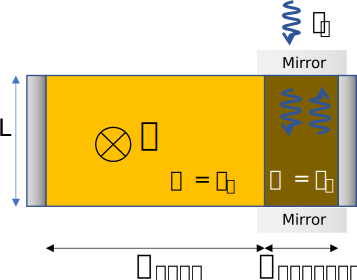
\includegraphics[]{\repodir/final/figures/schematics/output/contact_targeting.png} 
    \caption{Schematic of the contact targeting concept}
    \label{fig:SI_contact_targeting_schematic}
\end{figure}


To model both bulk and contact-targeted non-equilibrium generation, we only include non-equilibrium ionization in a fraction of the channel as shown in Figure \ref{fig:SI_contact_targeting_schematic}. The system comprises a bulk channel region of width $w_{b}$ and conductivity $\sigma_{b}$, and a boundary layer region near the contact of width $w_{c}$ and conductivity $\sigma_{c}$. By considering the series resistance of this 1D channel, the channel can be considered to have an effective conductivity, $\sigma_{eff}$, which can be shown to be:  

\begin{equation}
\sigma_{eff}=\frac{\sigma_{b} \sigma_{c}}{\sigma_{b}+l_{b}  (\sigma_{c}  -\sigma_{b})}
\end{equation}

Where we have defined the fractional bulk region width $l_{b}=w_{b}/(w_{c}+w_{b})$. The conductivities of the two regions are determined by setting two different gas temperatures and non-equilibrium generation conditions, as discussed below. In the limit of $l_{b}\rightarrow1$ and $l_{b}\rightarrow0$, the effective conductivity takes on the value $\sigma_{eff}= \sigma_{b}$ and $\sigma_{eff}= \sigma_{c}$, respectively. We can then model the case of uniform ionization of the entire channel by letting $l_{c}\rightarrow1$ so that $\sigma_{eff}= \sigma_{c}$.

To calculate $\gamma$, we use the chain rule, giving
\begin{equation}
\gamma_{c}=\frac{dP_{MHD}}{d\sigma_{eff}} \frac{d\sigma_{eff}}{d\sigma_{c}} \frac{d\sigma_{c}}{dn_e} \frac{dn_e}{dP_{in}}=\gamma \frac{d\sigma_{eff}},{d\sigma_{c}} 
\end{equation}
where we have recognized that this expression is equivalent to $\gamma$ in Equation \ref{eq:gamma-final} except for an "enhancement" factor $\frac{d\sigma_{eff}}{d\sigma_{c}}$. Finally, we can calculate $\frac{d\sigma_{eff}}{d\sigma_{c}}$ to be
\begin{equation}
\frac{d\sigma_{eff}}{d\sigma_{c}}=\frac{\sigma_{b}^2 (1-l_{b})}{[\sigma_{b}+l_{b} (\sigma_{c}-\sigma_{b})]^2} .
\end{equation}

%https://www.wolframgamma.com/input?i=derivative+of+%28b*c%29%2F%28b%2B+l+%28c++-b%29%29+with+respect+to+c

In the main text and figures below, we calculate $\frac{d\sigma_{eff}}{d\sigma_{c}}$ for a variety of different $T_{c}$ and setting $T_{b} = 3000$.

For cold boundary layers with small fractional width ($l_{b}\rightarrow1$), $\frac{d\sigma_{eff}}{d\sigma_{c}}$ can approach a factor of 100. However, if the boundary layer temperature is near the bulk temperature, $\frac{d\sigma_{eff}}{d\sigma_{c}}$ can actually be much less than 1. This indicates that contact targeting is only effective for $T_{c} \ll T_{b}$. 

It is still possible to have a $\frac{d\sigma_{eff}}{d\sigma_{c}}$ of less than 1 even if $T_{c} \ll T_{b}$ is the fractional width of the boundary layer is large and the  boundary layer temperature is near the bulk temperature. In this situation, changes in the boundary layer conductivity have a small effect on the effective conductivity. While the enhancement viability $\gamma$ is lowered in this situation, the absolute efficiency of the generator will be larger than for the case of a larger boundary layer width.

\begin{figure}[h]
    \centering
    \includegraphics[]{\repodir/modeling/viability/analysis/output/figures/bl_enhance.png} 
    \caption{Enhancement factor for contact targeting versus fractional bulk region width $l_b$}%DN: Is "enhancement factor" the same as "enhancement viability" the same as "viability figure of merit" \gamma?
    \label{fig:SI_bl_enhance}
\end{figure}

\clearpage

\subsubsection{Supplemental PI Viability Results}

\begin{figure}[h]
    \centering
    \includegraphics[width=0.8\linewidth]{\repodir/modeling/viability/figure_panels/output/P_zero_rxn_component.png} 
    \caption{$P_{zero}$ calculated for various reactions. For each reaction, the reaction is considered to be the only recombination reaction, except for "mm\_sum" where the sum over experimental O2, K+, H2O, and OH mono-molecular recombination rates is used.}
    \label{fig:SI_P_zero_rxn_component}
\end{figure}


\begin{figure}[h]
    \centering
    \includegraphics[width=0.8\linewidth]{\repodir/modeling/viability/figure_panels/output/viability_kwt.png} 
    \caption{$P_{zero}$ calculated for various potassium mass fractions. }
    \label{fig:SI_P_zero_kwt}
\end{figure}

% $krm_{O2_exp_eff} + 2*krm{K+} + krm_{H2O} + krm_{OH}$

% \begin{figure}
% \centering
% \includegraphics[width=\textwidth]{\repodir/modeling/viability/figure_panels/output/beta_boundary_layer.png}
% \caption{Supplemental results}
% \end{figure}

% \begin{figure}
% \centering
% 
\includegraphics[width=\textwidth]{\repodir/final/figures/SI/output/Viability_rxn_compare.png}
% \caption{Supplemental results}
% \end{figure}


